\documentclass{article}
\usepackage{listings}
\usepackage{graphicx}
\title{Urban area analysis using Statistics for SAR Imagery report}
\author{Zheng Wen}
\date\today
\begin{document}	
\maketitle
	\section{Data select}
	\begin{lstlisting}[frame=tb]
	
	The urban_area image in this report is select from 
Fig.3.4,in which we choose subimage of 100pixels * 100pixels
in urban area and show as Figure 1.In this experiment ,
we only select raw intensity HH bands as our objective.So the 
codes is very simple and understandable.

> #The road of raw intensity HH bands#
> imagepath <- "/home/a421-2/wenzheng/Report-Statistics-SAR-master
 /Data/Images/ESAR/"
> HH_Complex <- myread.ENVI(paste(imagepath,
				"ESAR97HH.DAT", sep = ""), 
				paste(imagepath, "ESAR97HH.hdr", sep = ""))
> HH_Intensity <- (Mod(HH_Complex))^2
> #The area of selected#
> urban_area <- HH_Intensity[1100:1199,1100:1199]
> vexample <- data.frame(HH=as.vector(urban_area))
	
> plot(imagematrix(equalize(urban_area)))
> imagematrixPNG(name = "./urban_area.png", imagematrix(equalize(urban_area)))
	
> vexample <- data.frame(HH=as.vector(urban_area))

> summary(vexample)
HH          
Min.   :       3  
1st Qu.:   16028  
Median :   51070  
Mean   :  193548  
3rd Qu.:  181281  
Max.   :11946965

	\end{lstlisting}

	\begin{figure}[htbp]
		\centering
		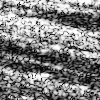
\includegraphics[width=0.5\linewidth]{urban_area.png}
		\caption{selected area}
		\label{fig:urban_area}
	\end{figure}

	\section{Analysis of Histogram}
	\begin{lstlisting}[frame=tb]
	
	Consider the real part of the HH band of Figure 2 and Figure 3 
whose histogram is the top leftmost. assume it is stored 
in the |HH_Complex| variable.These data are clearly not 
uniformly distributed.
	We will randomly sample (fixing the pseudorandom number 
generator and the seed for reproducibility) one hundred 
observations, and then proceed to build its empirical function.
	
>binwidth_complete <- 2*IQR(vexample$HH)*length(vexample$HH)^(-1/3)

>ggplot(data=vexample, aes(x=HH)) + 
			geom_histogram(aes(y=..density..), 
			binwidth = binwidth_complete) + 
			xlab("Intensities") +
			ylab("Proportions") +
			ggtitle("Complete Histogram") +
			theme_few()
>ggsave(filename = "./HistogramExample.pdf")

> binwidth_complete
[1] 15340.79

	\end{lstlisting}
	\begin{figure}
		\centering
		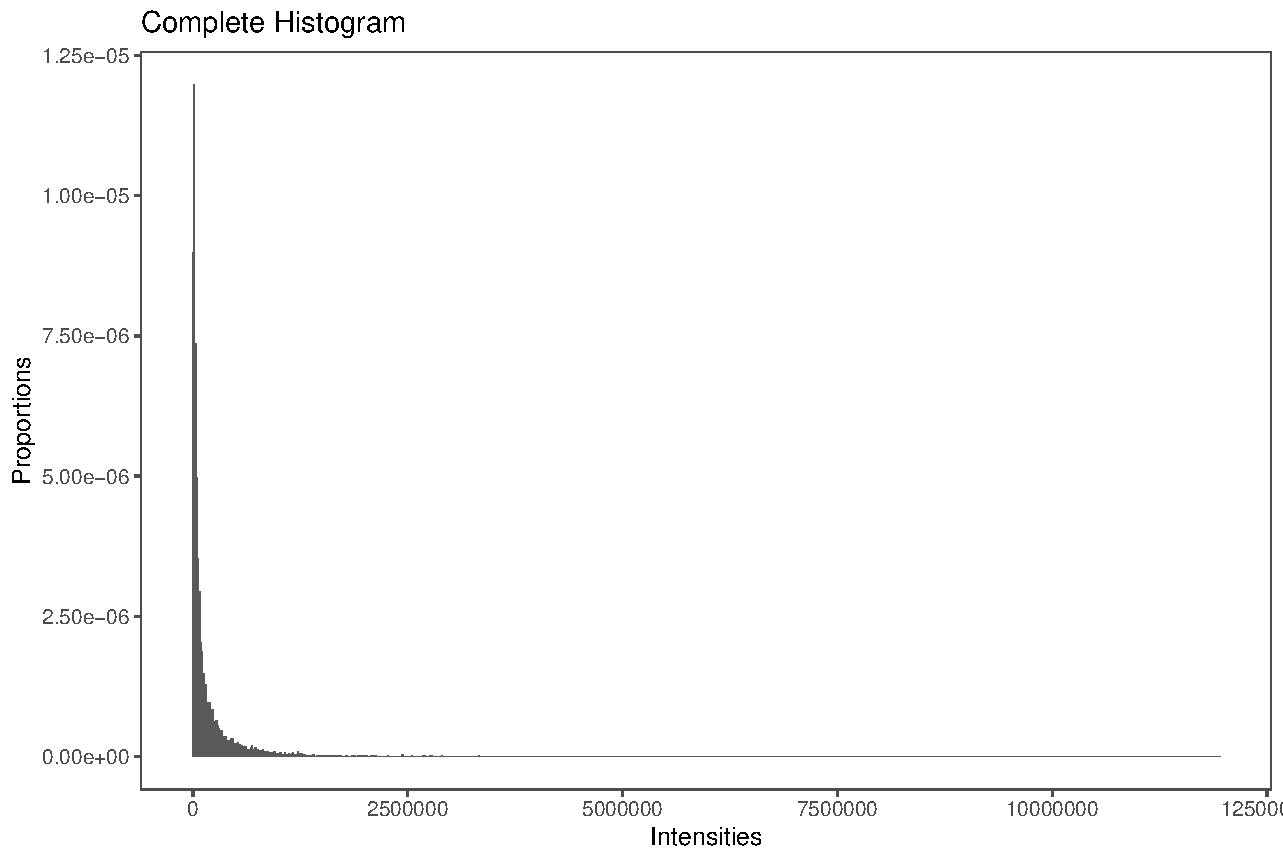
\includegraphics[width=1\linewidth]{HistogramExample.pdf}
		\caption{HistogramExample}
		\label{fig:HistogramExample}
	\end{figure}
	\begin{figure}
		\centering
		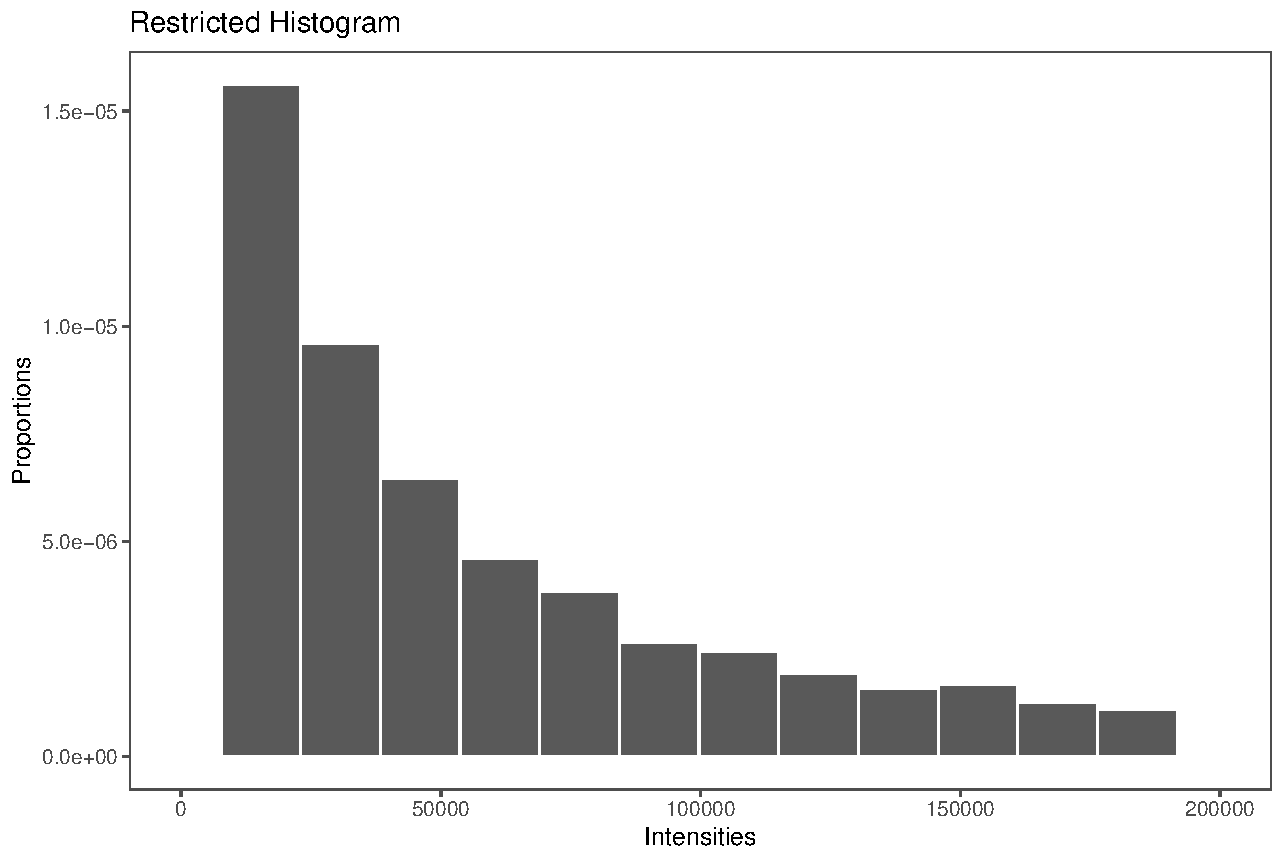
\includegraphics[width=1\linewidth]{HistogramRestrictedExample.pdf}
		\caption{HistogramRestrictedExample}
		\label{fig:HistogramRestrictedExample}
	\end{figure}


	\section{The result of estimation}
	\begin{lstlisting}[frame=tb]
	
	The maximum likelihood estimation is used to evaluate the 
experimental data. Here we use only one function to achieve 
this function, and eventually we get a result value.

## Estimation
require(maxLik)

GI0.Estimator.m1m2 <- function(z, L) {
			m1 <- mean(z)
			m2 <- mean(z^2)
			m212 <- m2/m1^2

			a <- -2 - (L+1) / (L * m212)
			g <- m1 * (2 + (L+1) / (L * m212))

return(list("alpha"=a, "gamma"=g))
}

estim.urban_area <- GI0.Estimator.m1m2(urban_area, 1)

LogLikelihoodLknown <- function(params) {

			p_alpha <- -abs(params[1])
			p_gamma <- abs(params[2])
			p_L <- abs(params[3])

			n <- length(z)

return(
n*(lgamma(p_L-p_alpha) - p_alpha*log(p_gamma) - lgamma(-p_alpha)) + 
		(p_alpha-p_L)*sum(log(p_gamma + z*p_L)) 
		)
}

estim.exampleML <- maxNR(LogLikelihoodLknown, 
start=c(estim.urban_area$alpha, estim.urban_area$gamma,1), 
activePar=c(TRUE,TRUE,FALSE))$estimate[1:2]

values:
binwidth_complete : 15340.7948389499
estim.exampleME : num [1:2] -42741 143335
mean : 1
N : 15
sigma2 : 1


> GI0.Estimator.m1m2
function(z, L) {
m1 <- mean(z)
m2 <- mean(z^2)
m212 <- m2/m1^2

a <- -2 - (L+1) / (L * m212)
g <- m1 * (2 + (L+1) / (L * m212))

return(list("alpha"=a, "gamma"=g))
}
<bytecode: 0x5566609e2b40>
> estim.urban_area
$alpha
[1] -2.279272

$gamma
[1] 441148

> estim.exampleML
[1] -42740.89 143335.12

	\end{lstlisting}
results all above
\end{document}


